\subsubsection*{Framework research}
% Il problema di questi framework è che comunque nascono l'infrastruttura sottostante e la
% gestiscono loro sotto, dando un accesso solo tramite API in maniera limitata.


Since PAPS focuses on serverless function, initially the research looked for a framework 
that would allow the user to create in a immediate way functions and would give the opportunity to manage their
deployment and placement inside the network.
In this way, the creation of containers is sped up, because the framework automates all the process
of creating a container and eliminates the need of adding useless boilerplate code.
\par
The first candidate was OpenWhisk \cite{OpenWhisk}, a serverless platform able to run 
functions on top of an existing infrastructure. The idea was to integrate it on top of a Kubernetes 
cluster, running a series of docker \cite{Docker} containers. \\
Searching on the internet information about the integration of those platforms, other two 
options were available: OpenFaas \cite{Faas} and Kubeless \cite{Kubeless}. For what concerns 
the functionalities the three frameworks are pretty similar one to another.
They all provide a mechanism to deploy functions that can be written in various programming languages.
These functions accept arguments and give a response in the form of a json file, whose structure
is determined by the programmer. In this way the mechanisms that deploy and call the functions are language agnostics.
\par
Function calls are controlled with Triggers, components that reacts to certain events inside the 
ecosystem (such as HTTP request or the call of another function).
OpenWhisk offers a very detailed protocol on how to design triggers, functions, and rules
that connect these two elements.
On the other hand, OpenFaas is less focused on this functionality and more oriented on HTTP calls.
\par
Kubeless stands out since it has a built-in synergy with Kubernetes. In order to support the creation of functions, 
it extends the Kubernetes API by creating a CustomResourceDefinition, a RESTful resource that is saved inside the Kubernetes
system. This new type of resource can be accessed like any other normal object inside Kubernetes
by making REST calls (via CLI or HTTP request).

\par
The main issue with OpenWhisk and Kubeless is 
that they are written in Scala and Akka; OpenWhisk also has a complex structure and for that reason 
is not optimal for a project like this. For what concerns OpenFaas, it is written
in Go and offers some additional features like a metrics system and the possibility to 
customize the scheduling policy used by the framework.
\\
During the research process one main  problem came out: all the frameworks hide to the final user 
the underlying infrastructure, making the integration of PAPS functionalities hard.
To solve this issue, the best decision was to build something directly on top of Kubernetes
using the provided API, available for a large variety of languages, to create, manage and 
delete containers when needed. \\
For what concerns the framework, OpenFaas came in handy to provide a frontend module 
useful for PAPS users which will be easily able to upload the functions that PAPS
will manage and distribute. We chose OpenFaas since it offers both a
simple UI and the possibility to be managed by a CLI. It was also the only one that offered the possibility to 
install a statistics collection module, which can be used to monitor how the
system is working in a real environment.


\subsubsection*{OpenFaas}
OpenFaas is a serverless framework that does not manage the infrastructure, since it delegates
this task to other IaaS frameworks (such as Kubernetes).
It works at the application level, easing the creation, management and deployment of functions
on the cluster. 
\par
A function is a piece of software that provides some functionality, receiving request and sending response
in a json file format. It will be deployed in the cluster in the form of multiple containers,
on which the user has no direct control or knowledge.
This allows the user to have a high level view of its functions, without having
to worry about the complexity of the management of the infrastructure, since functions and containers are decoupled.
\par
For what concerns the architecture, the main component of OpenFaas is the \textbf{API-gateaway}.
It exposes the REST-API that allows the user to manage its functions.
Both function calls and management requests are sent to the gateaway, which in turn will provide
to contact the right component in order to perform the desired action.
The API-gateaway can be invoked via CLI, UI or HTTP requests.
\\
When a function is deployed, on or more pods/containers are created. The \textbf{WatchDog}
is the component that is responsible for starting and monitoring functions. It becomes
an init process with an embedded HTTP server, and can support concurrent requests, timeouts and
healthchecks.
\\
The \textbf{Alert Manager} controls the traffic to which the function are subjected.
This is done monitoring the metrics produced by Prometeus. When the current configuration
cant keep up with the current workload or too much containers are allocated, the Alert Manager
fires an alert to the API-gateaway, that will provide to change accordingly the number of containers.
\\
All these components are builded on the cluster as standalone containers, and so they can be also
duplicated depending on the cluster administrator needs.

\subsubsection*{Kubernetes integration}
Kubernetes is an orchestration framework that automates deployment, scaling and management of containerized
applications on a multi-node cluster.
The containers are bundled in particular entities, Pods, that contain all the dependencies and 
additional metadata about the deployment. A set of controllers allows the user to automate
in a flexible way the deployment of these pods.
\\
Kubernetes offers to the user REST API, through which all object can be created, read, updated
and deleted. This object are stored inside the system and describe the desired state of the cluster.
\\
All objects have a metadata field, in which labels can be added and removed.
Labels can be used to mark an object, and their meaning is defined by the programmer that created it.
Labels allows filtering while asking for resources, and so they can be used to assign a particular role 
or attribute to a certain object.
\par
The infrastructure is managed with the help of some key components, that are divided into two categories:
Control Plane components and Kubernetes Node components.
\begin{figure}
    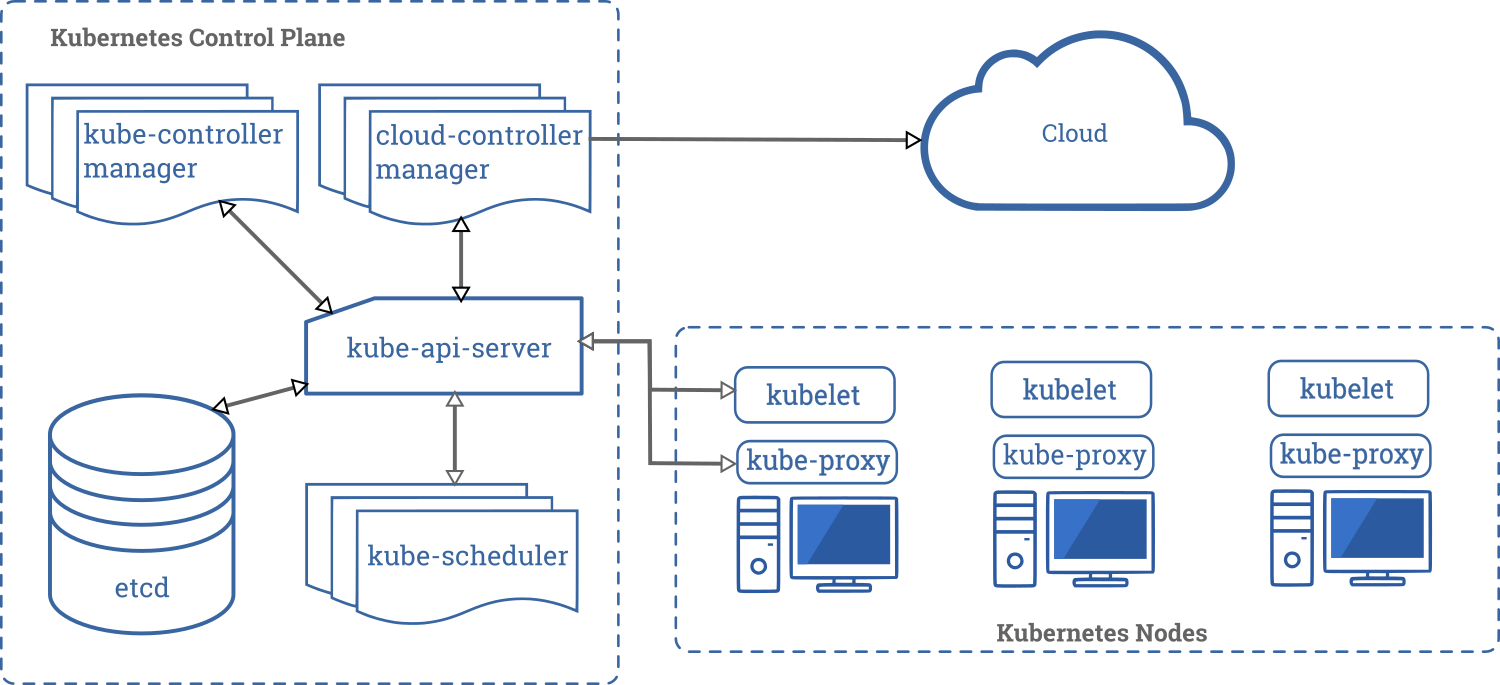
\includegraphics[width=\linewidth]{images/components-of-kubernetes.png}
    \caption{Components of Kubernetes.}
    \label{fig:boat1}
  \end{figure}


The \textbf{Control Plane components} has the role of managing the cluster, by making global decisions.
It detects and responds to cluster events. These components can be run on any machine, but usually
they are placed on a node called Master.
The \textbf{kube-api-server} is the frontend for the Kubernetes Control Plane. It implements Kubernetes'
REST API, that can be accessed with a CLI or an HTTP request. It allows to create and manage resources,
giving fine grained information about the cluster.
\\
The \textbf{etcd} is a key-value based storage, in which all the data about the cluster are saved.
\\
The \textbf{kube-scheduler} is notified when a pod has been created. Its function is to place this pod
on a node, taking into account some factors such that individual and collective resource
requirements, hardware/software/policy constraints, affinity and anti-affinity specifications,
data locality, and inter-workload interference.
The default scheduler can be replaced with a custom scheduler. A schedule routine
is composed of two phases. The \textit{Filtering} phase has the objective to identify a set 
of candidates nodes on which the pod can be scheduled, while in the \textit{Scoring} phase
a score for each node is calculated with the help of some heuristics. The node with the highest score
is the one that will host the given pod.
This two phases are ignored if the current pod has already specified in its fields the node
in which it will be scheduled.
\\
The \textbf{kube-controller-manager} runs all controller processes that manage both nodes and 
pods. The \textit{Node controller}
checks the status of the nodes in the cluster, responding accordingly if a node fails.
The \textit{Replication controller} controls all the pods, and reacts to changes of the pod number
by allocating or de-allocating accordingly to the desired state and the workload. If a node fails, all 
the pods that were active on it will be placed again thanks to its routines.
\par 
The \textbf{Kubernetes Node components} are placed on the node of the cluster and handle
the real creation and destruction of the containers.
\textbf{Kubelet} makes sure that containers are running in a Pod. It receives from the kube-api-server
a PodSpec (an object that describes all the dependencies and characteristics of the pod that
will run on the node) and checks if the containers described are running and healthy.
Kubelet does not manage containers that have been created outside of Kubernetes.
\\
The \textbf{kube-proxy} allows nodes to communicate with the api server. It maintains network rules,
allowing pods to communicate with one another.
\\
The \textbf{Container Runtime} is the software responsible for running containers.
\newline
\newline
\textbf{STA PARTE MI SA CHE E' DA SPOSTARE}
\textit{This feature can be used in PAPS to perform the partition of the network in communities.
In fact, Kubernetes doesn't hide the structure of the cluster, and allows to obtain information about
the hosts running through the Node object. Each Node correspond to an actual host that is
connected to the cluster, and therefore can be managed by Kubernetes. 
Every Node can be marked with two labels, "COMMUNITY" and "ROLE". The former assigns to the node 
the PAPS community to which it belongs, while the latter specifies if the host is the leader of the
community or just a member that executes the leader's allocation plan.
By filtering on these labels, all the nodes of a community can be retrieved, easing the tasks performed 
by the Allocation and Partition modules.}